\section{Bedienungsanleitung und GUI}
\label{sec:frontend}

Im Folgenden wir die Installation und die Bedienung des Programmes erläutert, sowie der Aufbau der Oberfläche beschrieben. Das Programm kann unter \url{https://dev.spline.de/svn/CommonUnfold/trunk/} runtergeladen\footnote{\texttt{\$ svn checkout \url{https://dev.spline.de/svn/CommonUnfold/trunk/}}} werden. Im Ordner \texttt{src} muss die Datei \texttt{common\_unfolding\_draw.py} mit dem folgenden Befehl gestartet werden:\\

\centerline{\texttt{\$ python common\_unfolding\_draw.py\\}}


Wird das Programm gestartet, so befindet man sich im Startfenster (siehe~Abb.~\ref{fig:startFenster}). Über den Menüeintrag \texttt{File} können ersteinmal neue Schachteln erzeugt werden (\texttt{New By Surface, New By Dimension}) oder gespeicherte Arbeiten geöffnet werden (\texttt{Open File - Ctrl+O}).

\begin{figure}[htbp]
  \centering
  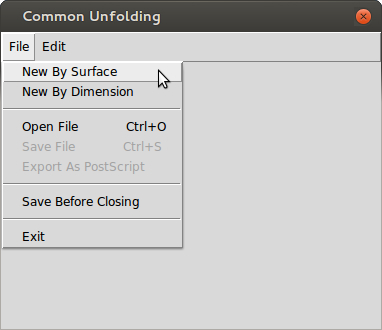
\includegraphics[scale=0.5]{03_pics/start.jpg}
  \caption{Startfenster}
  \label{fig:startFenster}
\end{figure}


%%%%%%%%%%%%%%%%%%%%%%%%%%%%%%%%%%%%%%%%%%%%%%%%%%%%%%%%%%%%%%%%%%%%%%%%%%%%%%%
%%%%%%%%%%%%%%%%%%%%%%%%%%%%%%%%%%%%%%%%%%%%%%%%%%%%%%%%%%%%%%%%%%%%%%%%%%%%%%%
%%%%%%%%%%%%%%%%%%%%%%%%%%%%%%%%%%%%%%%%%%%%%%%%%%%%%%%%%%%%%%%%%%%%%%%%%%%%%%%
% SCHACHTELN ERZEUGEN %%%%%%%%%%%%%%%%%%%%%%%%%%%%%%%%%%%%%%%%%%%%%%%%%%%%%%%%%
%%%%%%%%%%%%%%%%%%%%%%%%%%%%%%%%%%%%%%%%%%%%%%%%%%%%%%%%%%%%%%%%%%%%%%%%%%%%%%%
\subsection{Erzeugen von Schachteln}
\label{subsec:schachteln}

Die Anzahl der Schachteln kann man beim Erzeugen von neuen Schachteln frei wählen, \dH es können auch mehr als zwei Grundflächen ausgewählt werden. Aus dem sich ergebenden Commin-Unfold soll es möglich sein, die zuvor ausgewählten Schachteln zu falten. Bei der Erzeugung von neuen Schachteln, kann zwischen \texttt{New By Surface} und \texttt{New By Dimension} gewählt werden.

  \begin{description}
    \item [{New~By~Surface:}] Hier gibt man den Oberflächeninhalt an. Gibt es mehr als eine Schachtel, welche diesen Oberflächeninhalt hat, so werden diese erzeugt. Beispielsweise erzeugen die Oberflächeninhalte $22, 30, 34, 38, 40$ und $42$ jeweils zwei verschieden dimensionierte Schachteln, die Oberflächeninhalte $46, 54$ und $58$ jeweils drei Schachteln.
    \item [{New~By~Dimension:}] Hier gibt man die Breite, Höhe und Tiefe einer Schachtel an, alle weiteren, die in die gleiche Äquvalenzklasse fallen, werden erzeugt. Funktionierende Beispiele dafür sind die Dimensionen $1\times1\times5$, $1\times2\times3$ und $1\times4\times5$.
  \end{description}

Alle Schachteln werden in einer \emph{Preview} angezeigt und stehen zur Auswahl (Checkboxen) in einem neuen Fenster bereit (siehe~Abb.~\ref{fig:preview}). Man muss mindestens zwei Schachteln auswählen um das Programm zu starten. Existieren nur zwei Schachtel, werden diese automatisch Vorausgewählt. Zusätzlich kann man die Rotation der Schachteln in Grad angeben, diese werden dabei um ihren Urspungspunkt im Uhrzeigersinn rotiert.

\begin{figure}[htbp]
  \centering
  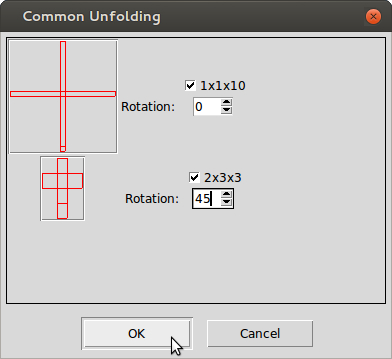
\includegraphics[scale=0.5]{03_pics/auswahl.jpg}
  \caption{Auswahlfenster für Schachteln}
  \label{fig:preview}
\end{figure}


%%%%%%%%%%%%%%%%%%%%%%%%%%%%%%%%%%%%%%%%%%%%%%%%%%%%%%%%%%%%%%%%%%%%%%%%%%%%%%%
%%%%%%%%%%%%%%%%%%%%%%%%%%%%%%%%%%%%%%%%%%%%%%%%%%%%%%%%%%%%%%%%%%%%%%%%%%%%%%%
%%%%%%%%%%%%%%%%%%%%%%%%%%%%%%%%%%%%%%%%%%%%%%%%%%%%%%%%%%%%%%%%%%%%%%%%%%%%%%%
% ZEICHENOBERFLÄCHE %%%%%%%%%%%%%%%%%%%%%%%%%%%%%%%%%%%%%%%%%%%%%%%%%%%%%%%%%%%
%%%%%%%%%%%%%%%%%%%%%%%%%%%%%%%%%%%%%%%%%%%%%%%%%%%%%%%%%%%%%%%%%%%%%%%%%%%%%%%
\subsection{Zeichenoberfläche und Startpunkte}
\label{subsec:zeichenoberflaeche}

Wählt man mehr als eine Schachteln aus und bestätigt die Auswahl mit \texttt{OK}, so gelangt man zur \emph{Zeichenoberfläche} (siehe~Abb.~\ref{fig:zeichenoberflaeche}). 

Die Zeichenoberfläche besteht aus den folgenden vier Bereichen:

  \begin{description}
    \item [{(1)~Zeichenbereich:}] In diesem Bereich wird gezeichnet, hier     entsteht die neue Grundfläche aus der die links angezeigten Schachteln   gefaltet werden können.
    \item [(2)~Netze~der~Schachteln:] Im linken Bereich der Oberfläche werden alle ausgewählten Gitternetze untereinander angezeigt.
    \item [(3)~Startpunkte-Dialog] Bevor man zeichnen kann, können Startpunkte auf den einzelnen Schachteln gesetzt werden, dies kann in einem extra Fenster passieren (es wird beim Erstellen der Schacchteln automatisch geöffnet), indem die genauen $(x,y)$-Werte für alle Schachteln eingegeben werden oder auch durch Klicken auf die Schachteln direkt im Bereich~(3). Das Setzen der Startpunkte auch über die Menüleiste \texttt{Edit $\rightarrow$ Set Start Points} erfolgen.
    \item [(4)~Werkzeugleiste] Hier können verschiedene Optionen bezüglich des Zeichenvorgangs eingestellt werden. Dazu gehören das Einstellen der Pinselgröße, Zeichenfarbe und Pinselform. Außerdem müssen \texttt{Overwrite}, \texttt{Autofill} und \texttt{Continue} noch erklärt werden. [TODO:XXX]
  \end{description}

\begin{figure}[htbp]
  \centering
  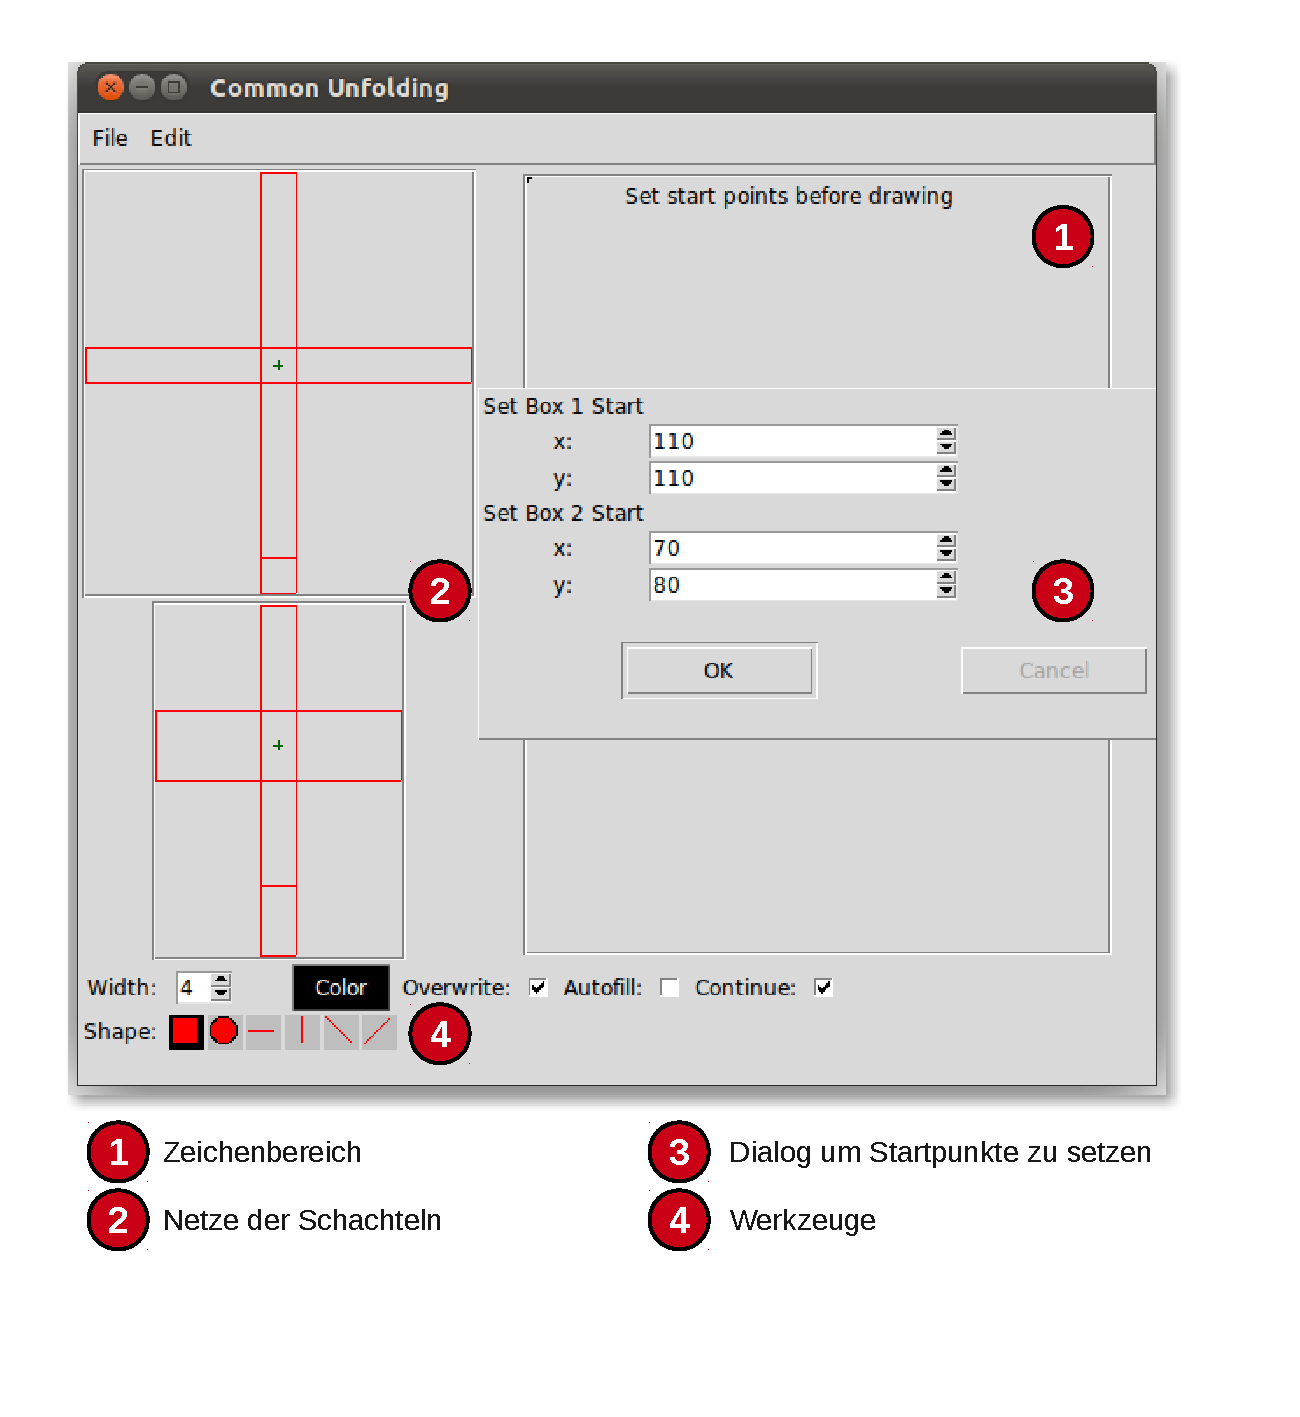
\includegraphics[scale=0.5]{03_pics/Zeichenbereich.pdf}
  \caption{Zeichenoberfläche}
  \label{fig:zeichenoberflaeche}
\end{figure}

[TODO:XXX:Bild an die anderen Bilder anpassen]


%%%%%%%%%%%%%%%%%%%%%%%%%%%%%%%%%%%%%%%%%%%%%%%%%%%%%%%%%%%%%%%%%%%%%%%%%%%%%%%
%%%%%%%%%%%%%%%%%%%%%%%%%%%%%%%%%%%%%%%%%%%%%%%%%%%%%%%%%%%%%%%%%%%%%%%%%%%%%%%
%%%%%%%%%%%%%%%%%%%%%%%%%%%%%%%%%%%%%%%%%%%%%%%%%%%%%%%%%%%%%%%%%%%%%%%%%%%%%%%
% DAS ZEICHNEN %%%%%%%%%%%%%%%%%%%%%%%%%%%%%%%%%%%%%%%%%%%%%%%%%%%%%%%%%%%%%%%%
%%%%%%%%%%%%%%%%%%%%%%%%%%%%%%%%%%%%%%%%%%%%%%%%%%%%%%%%%%%%%%%%%%%%%%%%%%%%%%%
\subsection{Das Zeichnen}
[TODO:XXX]


%%%%%%%%%%%%%%%%%%%%%%%%%%%%%%%%%%%%%%%%%%%%%%%%%%%%%%%%%%%%%%%%%%%%%%%%%%%%%%%
%%%%%%%%%%%%%%%%%%%%%%%%%%%%%%%%%%%%%%%%%%%%%%%%%%%%%%%%%%%%%%%%%%%%%%%%%%%%%%%
%%%%%%%%%%%%%%%%%%%%%%%%%%%%%%%%%%%%%%%%%%%%%%%%%%%%%%%%%%%%%%%%%%%%%%%%%%%%%%%
% LADEN, SPEICHERN, EXPORTIEREN %%%%%%%%%%%%%%%%%%%%%%%%%%%%%%%%%%%%%%%%%%%%%%%
%%%%%%%%%%%%%%%%%%%%%%%%%%%%%%%%%%%%%%%%%%%%%%%%%%%%%%%%%%%%%%%%%%%%%%%%%%%%%%%
\subsection{Datei lade, speichern, exportieren}
\label{subsec:dateioperationen}

Beschreibung wie werden Dateien geladen, gespeichert und exportiert.
[TODO:XXX]